\documentclass{article}
\usepackage{tikz}
\usetikzlibrary{arrows,shapes}
 
\begin{document}

%% you can give labels to the nodes, and can refer to them later.  
 
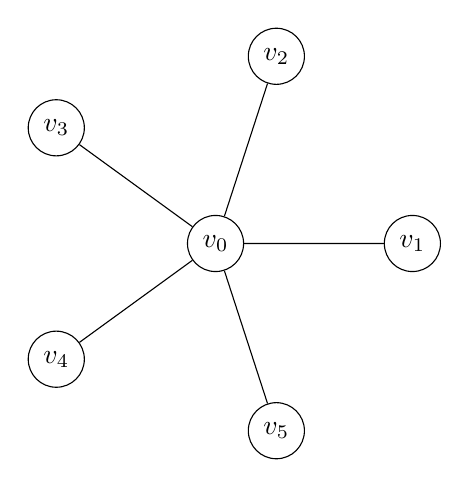
\begin{tikzpicture}[scale=2.5]
\tikzstyle{every node}=[draw,shape=circle];
\path (0:0cm) node (v0) {$v_0$};
\path (0:1cm) node (v1) {$v_1$};
\path (72:1cm) node (v2) {$v_2$};
\path (2*72:1cm) node (v3) {$v_3$};
\path (3*72:1cm) node (v4) {$v_4$};
\path (4*72:1cm) node (v5) {$v_5$};
\draw (v0) -- (v1)
(v0) -- (v2)
(v0) -- (v3)
(v0) -- (v4)
(v0) -- (v5);
\end{tikzpicture}


\end{document}
